This chapter will give the reader the necessary background knowledge
in order for this work to be understandable. First, it will go through
Apache Hadoop, a distributed storage and processing framework. We will
give some brief introduction to Hadoop file system (HDFS), then we
will dive into the
resource manager (YARN) and in what way Hops-YARN extend the Apache
YARN project. Later we will introduce a distributed, highly-available,
highly-redundant relational database, MySQL Cluster (NDB) and finally
we will give some insights on the different types of resource managing
systems.

In Figure \ref{fig:back_hpc_arch_overview} we can see a high level
overview of the architecture in HPC. Storage nodes are machines with very high disk capacity and bare
minimum processing power. Their main usage is to store data that are
going to be processed and analyzed in the future. The second building
block of the architecture is the Computing nodes. These machines have
no storage capabilities but they are equipped with the state of the art
processing units and a lot of RAM. Those modules communicate most
probably with a high throughput, low latency network. The most common
industry standard for interconnecting nodes in HPC is InfiniBand
\cite{infiniband} that can
reach 30 Gb/s in each direction and sub-microsecond latency. Users
issue their jobs to the Head node which is responsible for transferring
the requested datasets from the Storage nodes to the Computing nodes,
monitor the tasks and finally return the result to the end user.

\begin{figure}
\centering
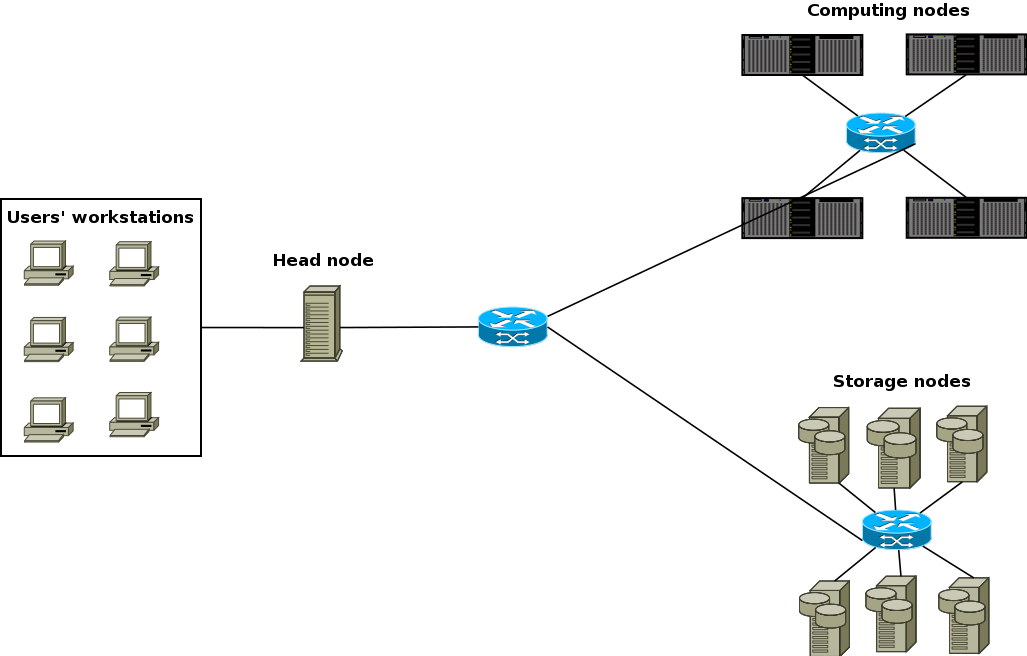
\includegraphics[scale=0.35]{resources/images/Background/hpc_arch_overview.png}
\caption{HPC high level architecture}
\label{fig:back_hpc_arch_overview}
\end{figure}

In 2003 Google published a paper describing GoogleFS (GFS)
\cite{Ghemawat:2003:GFS:1165389.945450}, a proprietary distributed
file system. It was designed to run on large clusters of commodity
hardware, that are doomed to fail at some time. That was the main
motivation that drove GFS to be fault-tolerant and
highly-available. Apache HDFS is the open-source implementation of GFS
and it will be analyzed in Section \ref{sec:hdfs}. In 2004 Google
published MapReduce \cite{Dean:2004:MSD:1251254.1251264}, a breakthrough programming model which exploited the locality
awareness of GFS and changed the way we process very big
datasets. MapReduce was later implemented for Hadoop and paved the way
for YARN, the current resource manager and scheduler 
which will be analyzed in Section \ref{ssec:yarn}.
